\documentclass[tikz]{standalone}

\usetikzlibrary{calc,positioning,shapes.geometric,backgrounds,fit,shadows.blur,arrows,arrows.meta,decorations.markings}

\newcommand*{\StrikeThruDistance}{0.15cm}%
\newcommand*{\StrikeThru}{\StrikeThruDistance,\StrikeThruDistance}%

\tikzset{strike thru arrow/.style={
    decoration={markings, mark=at position 0.5 with {
        \draw [blue, thick,-] 
            ++ (-\StrikeThruDistance,-\StrikeThruDistance) 
            -- ( \StrikeThruDistance, \StrikeThruDistance);}
    },
    postaction={decorate},
}}

\begin{document}
    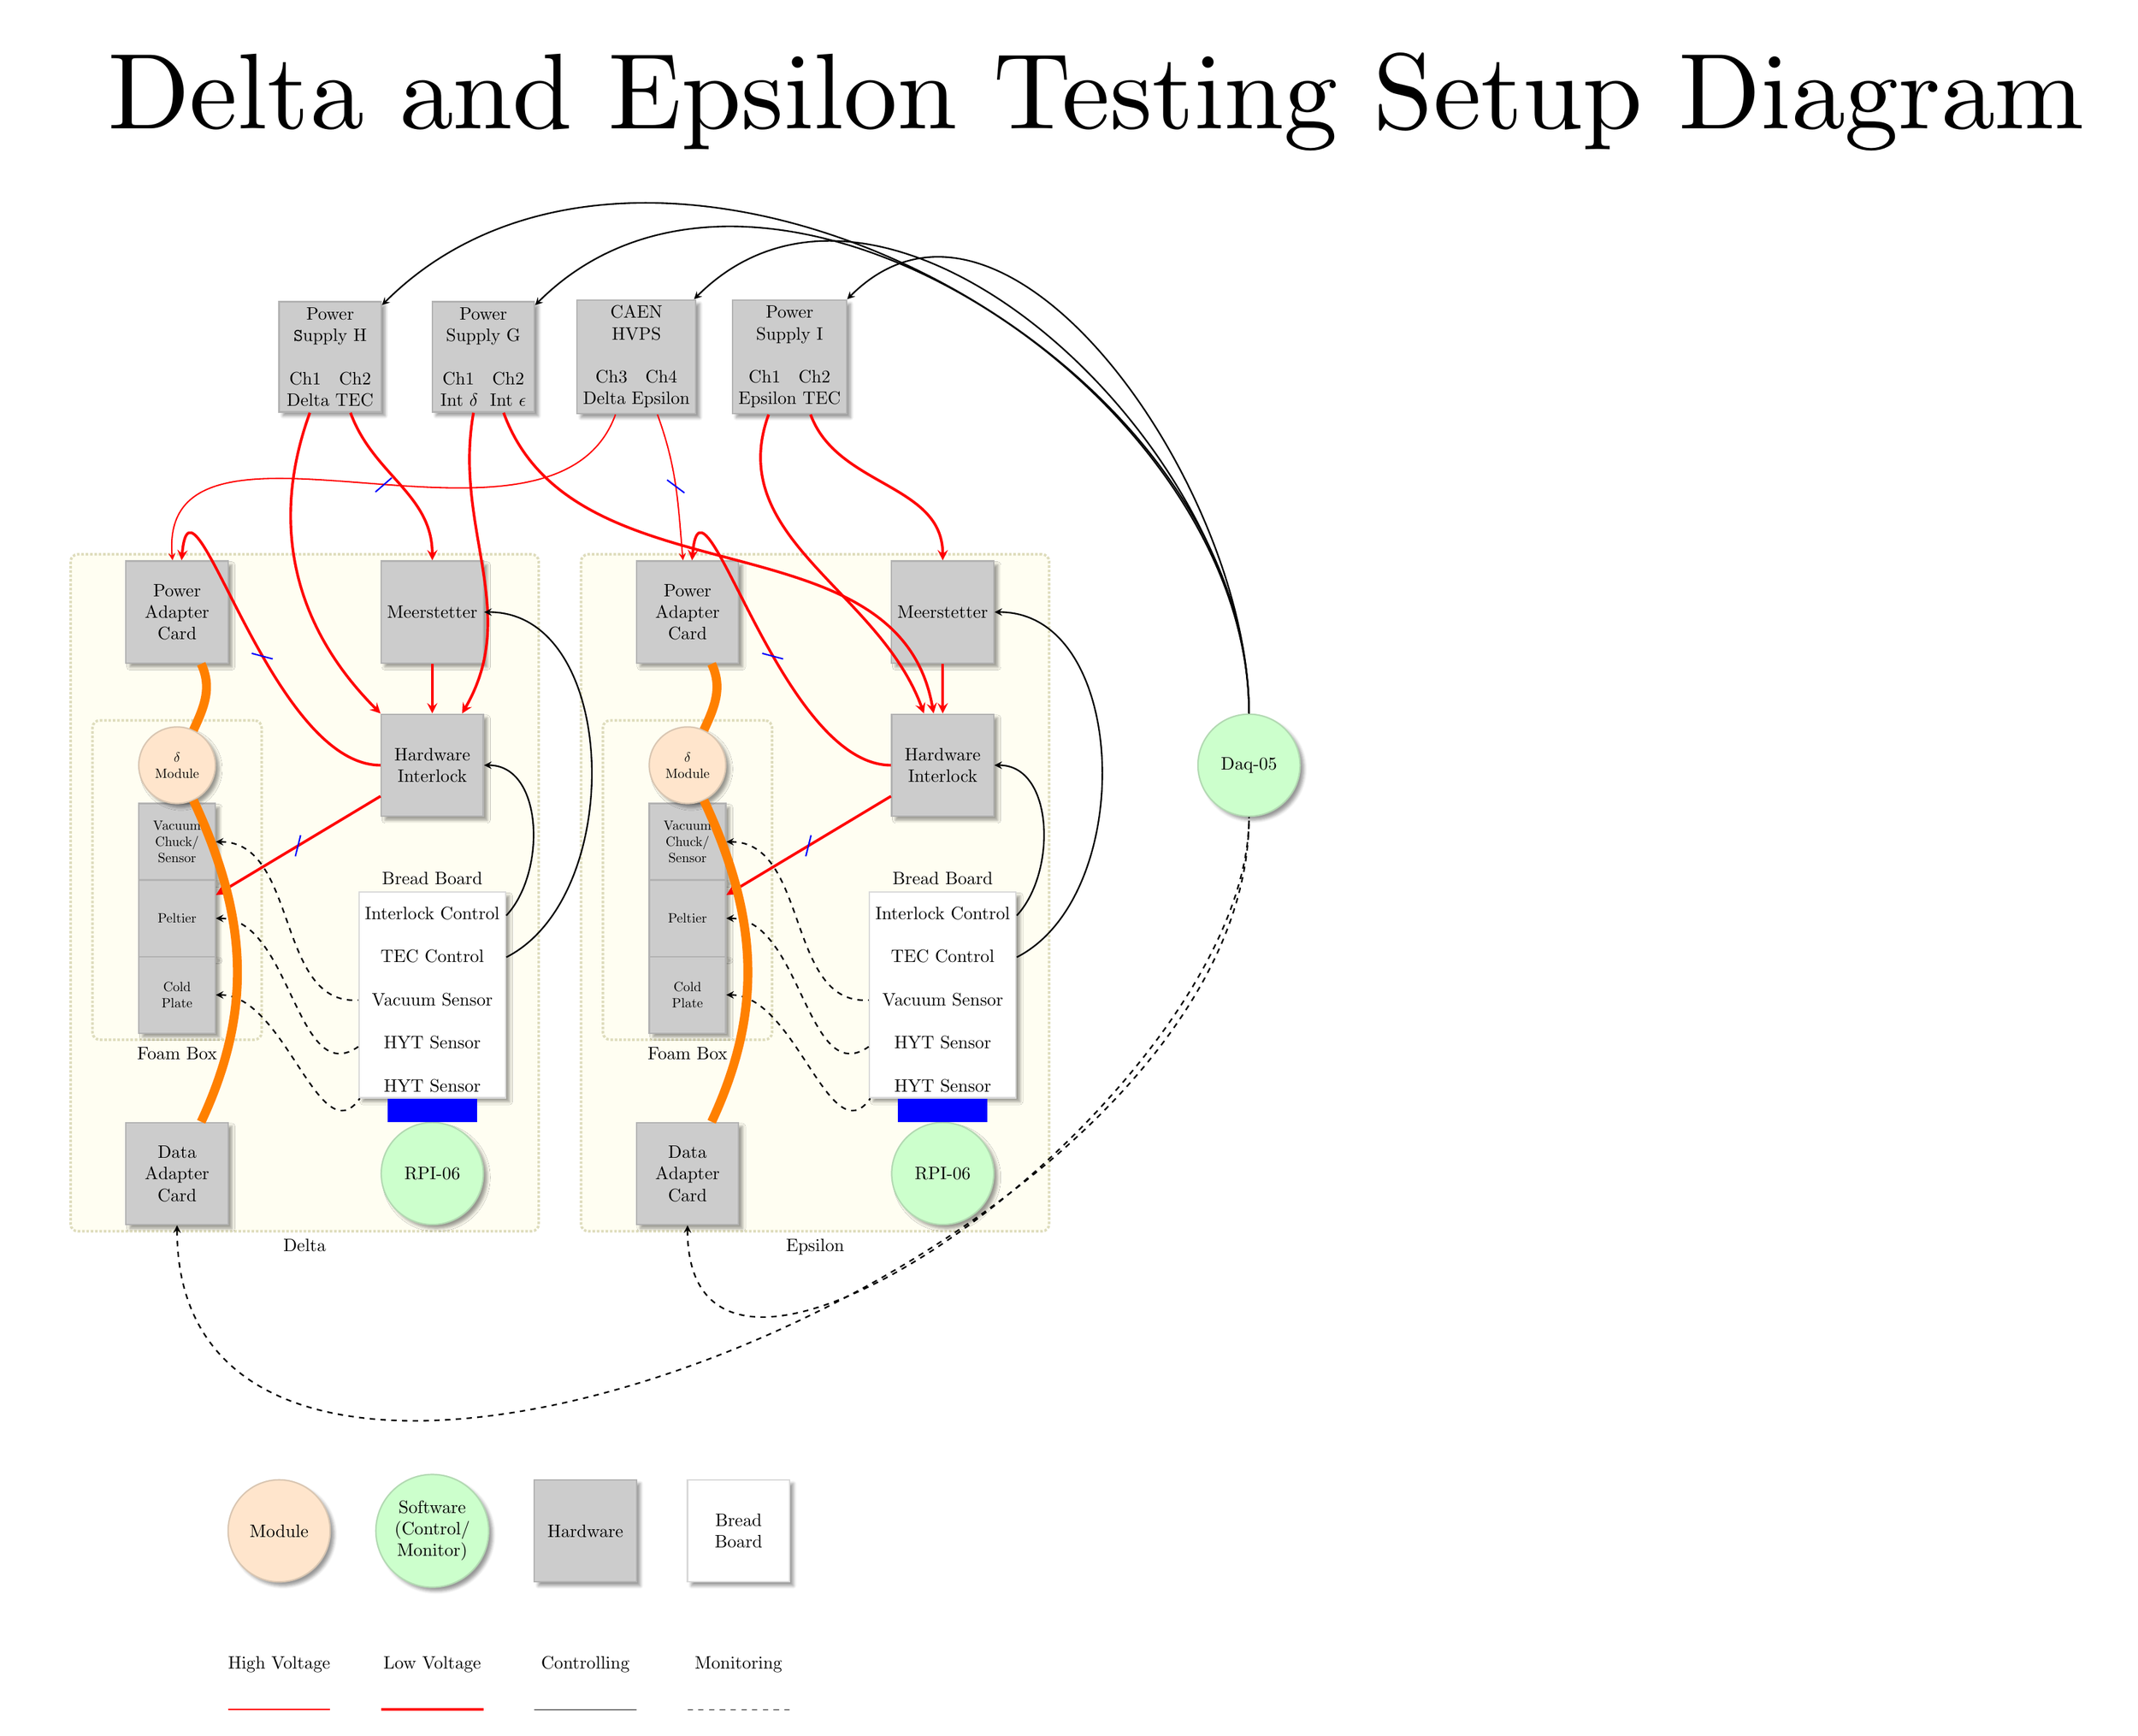
\begin{tikzpicture}[
	align=center,
        >=stealth,
        node distance=3cm,
	auto,
	line width=0.3mm,
        colorit/.style={
      	draw=#1!50!black!30,
      	fill=#1!20,
      	thick,
		blur shadow={shadow blur steps=5}
        },
        colorit/.default=black,
        database/.style={square, colorit=grey, shape border rotate=90, aspect=0.25, minimum size=2cm},
        software/.style={circle,colorit=green, minimum size=2cm},
	hardware/.style={rectangle,colorit=black, minimum size=2cm},
	module/.style={circle,colorit=orange, minimum size=2cm},
	database/.style={diamond,colorit=purple, minimum size=2cm},
	boxit/.style={
    	draw=#1!50!black!30,
		fill=#1!5,
		densely dotted,
		line width=0.5mm,
		rounded corners
	},
        bb/.style={rectangle,colorit=white, minimum size=2cm},
	boxit/.default=yellow
  	]
\begin{scope}[every node/.append style={scale=6}, node distance=2.5cm]
    \node at (20,10) {Delta and Epsilon Testing Setup Diagram};
\end{scope}
    % power supplies
    \node[hardware] at (5,5) (psh) {Power\\\texttt Supply H\\\texttt {}\\\texttt {}Ch1 { { }}Ch2\\\texttt{}Delta TEC};
    \node[hardware, right of = psh] (psg) {Power\\\texttt {}Supply G\\\texttt{}\\\texttt {}Ch1 { { }}Ch2\\\texttt{}Int $\delta${ { }}Int $\epsilon$};
    \node[hardware, right of = psg] (hvps) {CAEN\\\texttt {}HVPS\\\texttt {}\\\texttt {}Ch3 { { }}Ch4\\\texttt{}Delta Epsilon};
    \node[hardware, right of = hvps] (psi) {Power\\\texttt {}Supply I\\\texttt {}\\\texttt {}Ch1 { { }}Ch2\\\texttt{}Epsilon TEC};
    \node[software] at (23,-3) (daq) {Daq-05}
    edge[->, in = 45, out = 90] (psh)
    edge[->, in = 45, out = 90] (psg)
    edge[->, in = 45, out = 90] (hvps)
    edge[->, in = 45, out = 90] (psi);
    
    % delta
    \node[hardware] at (2,0) (pac) {Power\\Adapter\\Card}
    edge[<-, red, line width = 0.75, strike thru arrow, in = 250, out = 95] (hvps);
    \node[hardware] at (7,0) (meer) {Meerstetter}
    edge[<-, red, line width = 1.5, in = 290, out = 90] (psh);
    \node[hardware, below of = meer] (int) {Hardware\\Interlock}
    edge[<-, red, line width = 1.5, in = 250, out = 135] (psh)
    edge[<-, red, line width = 1.5, in = 260, out = 60] (psg)
    edge[->, red, line width = 1.5, strike thru arrow, in = 85, out = 180] (pac)
    edge[<-, red, line width = 1.5] (meer);
    \node[label=above:Bread Board, bb] at (7,-7.5) (bb) {\\{Interlock Control}\\{}\\{TEC Control}\\{}\\{Vacuum Sensor}\\{}\\{HYT Sensor}\\{}\\{HYT Sensor}}
    edge[->, in = 0, out = 27] (meer)
    edge[->, in = 0, out = 47] (int);
    \node[software] at (7,-11) (rpi) {RPI-06}
    edge[-, blue, line width = 50] (bb);
    \node[hardware] at (2,-11) (dac) {Data\\Adapter\\Card}
    edge[<-, dashed, in = 270, out = 270] (daq);
    
    % foam box
\begin{scope}[every node/.append style={scale=.75}, node distance=2cm]
    \node[hardware] at (2,-4.5) (chuck) {Vacuum\\Chuck/\\Sensor}
    edge[<-, dashed, in = 184, out = 0] (bb);
    \node[hardware, below of =chuck] (pelt) {Peltier}
    edge[<-, red, line width = 1.5, strike thru arrow] (int)
    edge[<-, dashed, in = 215, out = 0] (bb);
    \node[hardware, below of = pelt] (cp) {Cold\\Plate}
    edge[<-, dashed, in = 235, out = 0] (bb);
    \node[module, above of = chuck] (mod) {$\delta$\\Module}
    edge[-, orange, line width = 5, in = 295, out = 65] (pac)
    edge[-, orange, line width = 5, in = 65, out = 295] (dac);
\end{scope}
\begin{scope}[every node/.append style={scale=5}, node distance=2cm]
    \node[] at (2,-4) (oo) { { { { }}}};
    \node[] at (4.5,-4) (oo1) { { { { { { { { { { { { { { }}}}}}}}}}}}}};
\end{scope}

    % epsilon
    \node[hardware] at (12,0) (pac1) {Power\\Adapter\\Card}
    edge[<-, red, line width = 0.75, strike thru arrow, in = 290, out = 95] (hvps);
    \node[hardware] at (17,0) (meer1) {Meerstetter}
    edge[<-, red, line width = 1.5, in = 290, out = 90] (psi);
    \node[hardware, below of = meer1] (int1) {Hardware\\Interlock}
    edge[<-, red, line width = 1.5, in = 250, out = 110] (psi)
    edge[<-, red, line width = 1.5, in = 290, out = 100] (psg)
    edge[->, red, line width = 1.5, strike thru arrow, in = 85, out = 180] (pac1)
    edge[<-, red, line width = 1.5] (meer1);
    \node[label=above:Bread Board, bb] at (17,-7.5) (bb1) {\\{Interlock Control}\\{}\\{TEC Control}\\{}\\{Vacuum Sensor}\\{}\\{HYT Sensor}\\{}\\{HYT Sensor}}
    edge[->, in = 0, out = 27] (meer1)
    edge[->, in = 0, out = 47] (int1); 
    \node[software] at (17,-11) (rpi1) {RPI-06}
    edge[-, blue, line width = 50] (bb1);
    \node[hardware] at (12,-11) (dac1) {Data\\Adapter\\Card}
    edge[<-, dashed, in = 270, out = 270] (daq);
    % foam box
\begin{scope}[every node/.append style={scale=.75}, node distance=2cm]
    \node[hardware] at (12,-4.5) (chuck1) {Vacuum\\Chuck/\\Sensor}
    edge[<-, dashed, in = 184, out = 0] (bb1);
    \node[hardware, below of =chuck1] (pelt1) {Peltier}
    edge[<-, red, line width = 1.5, strike thru arrow] (int1)
    edge[<-, dashed, in = 215, out = 0] (bb1);
    \node[hardware, below of = pelt1] (cp1) {Cold\\Plate}
    edge[<-, dashed, in = 235, out = 0] (bb1);
    \node[module, above of = chuck1] (mod1) {$\delta$\\Module}
    edge[-, orange, line width = 5, in = 295, out = 65] (pac1)
    edge[-, orange, line width = 5, in = 65, out = 295] (dac1);
\end{scope}
\begin{scope}[every node/.append style={scale=5}, node distance=2cm]
    \node[] at (12,-4) (oo2) { { { { }}}};
    \node[] at (14.5,-4) (oo3) { { { { { { { { { { { { { { }}}}}}}}}}}}}};
\end{scope}
\begin{scope}[on background layer][every node/.append style={scale=1}, node distance=2cm]
    \node [label=below:Delta, boxit, fit= (oo1) (pac) (rpi)] {};
    \node [label=below:Foam Box, boxit, fit=(mod) (chuck) (pelt) (cp) (oo)] {};
    \node [label=below:Epsilon, boxit, fit= (oo3) (pac1) (rpi1)] {};
    \node [label=below:Foam Box, boxit, fit=(mod1) (chuck1) (pelt1) (cp1) (oo2)] {};
\end{scope}

    % legend
\begin{scope}[on background layer][every node/.append style={scale=1}, node distance=2cm]
    \node[module] at (4,-18) (modlegend) {Module};
    \node[software, right of = modlegend] (softlegend) {Software\\(Control/\\Monitor)};
    \node[hardware, right of = softlegend] (hardlegend){Hardware};
    \node[bb, right of = hardlegend] (bblegend) {Bread\\Board};
    \draw[-, red, line width=.75] (3,-21.5) -- (5,-21.5);
    \draw[-, red, line width=1.5] (6,-21.5) -- (8,-21.5);
    \draw[-] (9,-21.5) -- (11,-21.5);
    \draw[-, dashed] (12,-21.5) -- (14,-21.5);
    \node[below of  = modlegend] (hvlegend) {High Voltage\\{}\\{}};
    \node[right of = hvlegend] (lvlegend) {Low Voltage\\{}\\{}};
    \node[right of = lvlegend] (conlegend) {Controlling\\{}\\{}};
    \node[right of = conlegend] (monlegend) {Monitoring\\{}\\{}};
    \node[right of = monlegend]{};
    \node[left of = dac]{};
\end{scope}

\end{tikzpicture}

\end{document}
